\section*{Aufgabenstellung}

Die Brechzahl in einer bestimmten Glassorte beträgt für rotes Licht $n_{rot} = 1,51$ und für blaues Licht $n_{blau} = 1,52$. Auf ein Prisma, dessen Querschnittsfläche ein gleichseitiges Dreieck ist, fällt ein schmales Lichtbündel mit einem Einfallswinkel von $45 \degree$. Das Licht wird auf einem $2m$ entfernten Schirm aufgefangen. Berechnen Sie den Abstand des blauen und des roten Bereichs im Spektrum auf dem Schirm.



\section{Annahmen}

\subsection{Schirm}

Der Schirm sei gerade und weise gleiche Winkel zu den beiden äußersten Strahlen des Spektrums auf.

\section{Prisma}

Das Prisma sei so klein, dass der Unterschied der Austrittspunkte für die Strahlen unterschiedlicher Wellenlängen vernachlässigt werden können und Punkt S als uniformer Austrittspunkt der Strahlen aus dem Prisma. Die Winkel mit welchen das Licht auf den Punkt S auftrifft, werden jedoch berücksichtigt, da diese unabhängig von der Größe des Prismas sind.

\section{Zeichnung}	\label{sec:zeichnung}

\begin{figure}[ht!]
	\vspace{-15px}	
	\begin{center}
		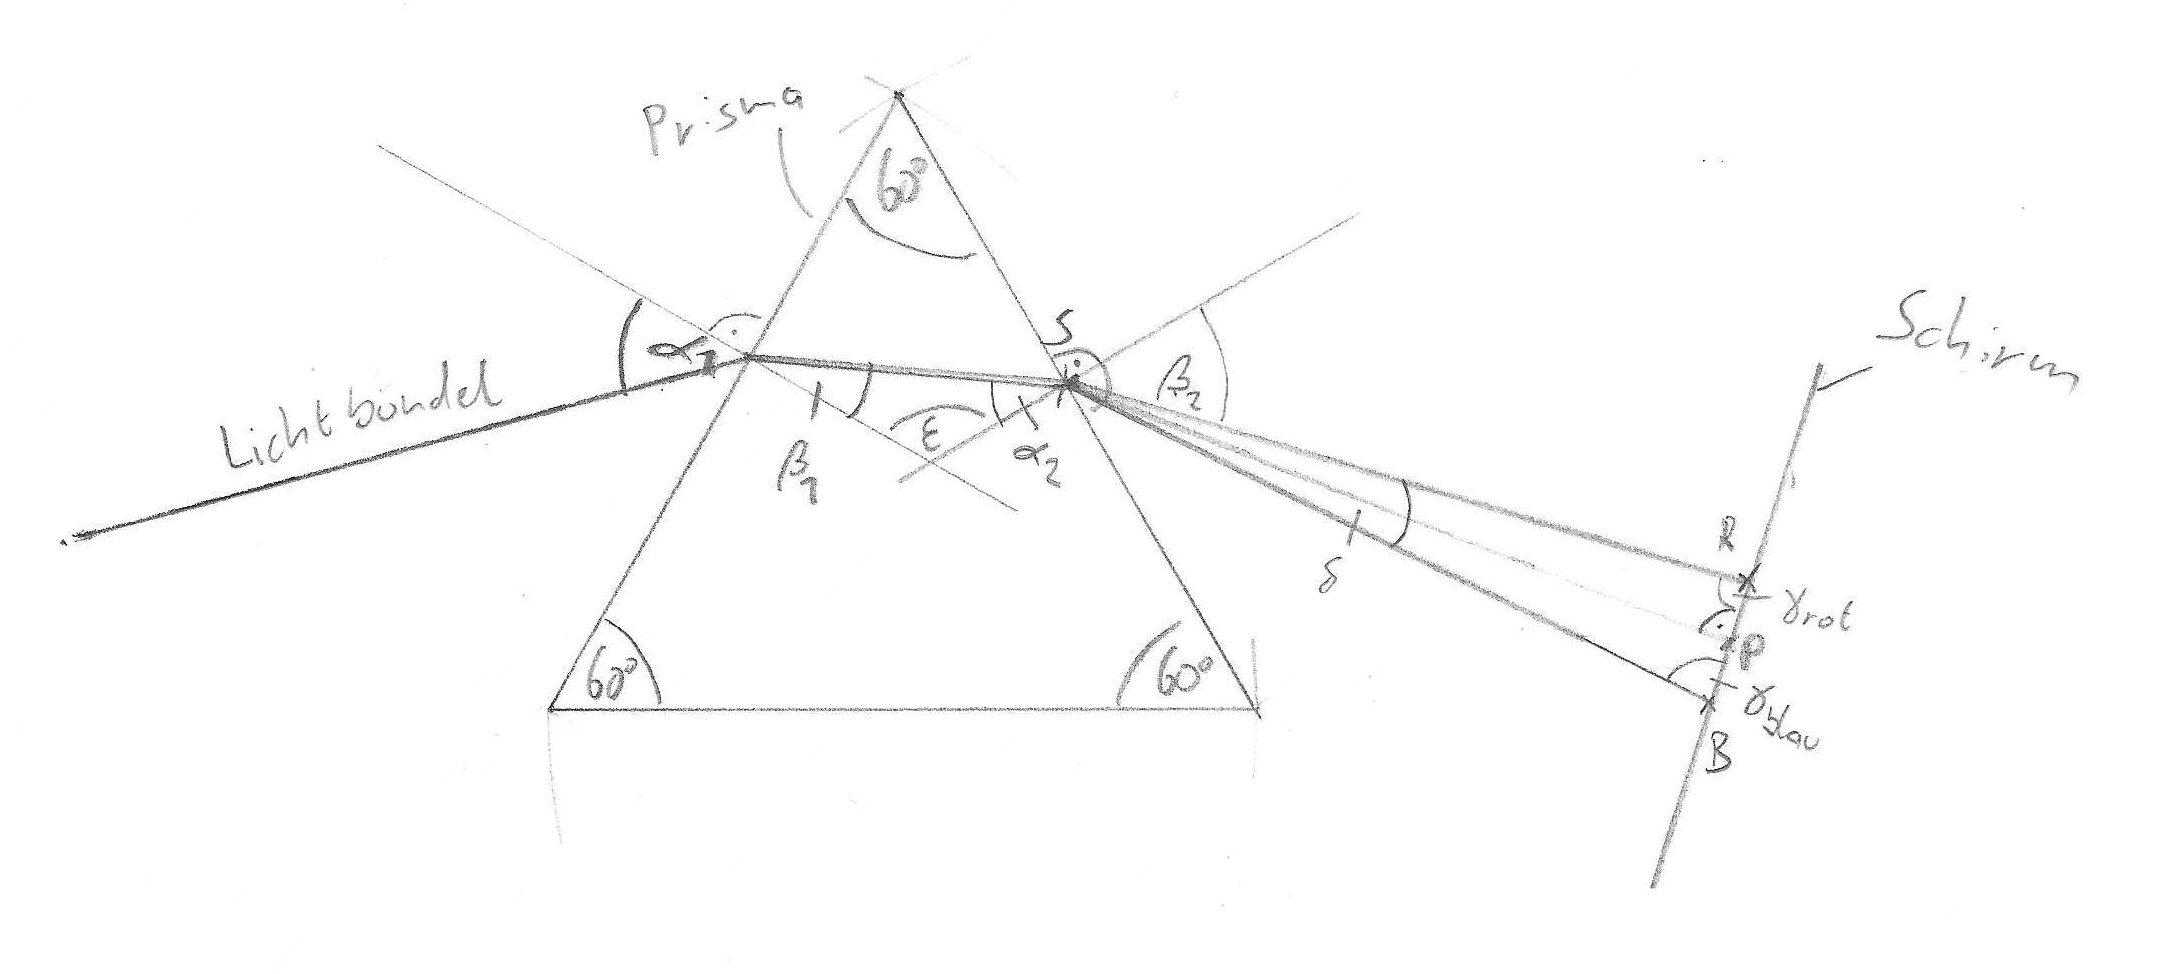
\includegraphics[width=0.9\textwidth]{skizze}
		\caption{Zeichnung}
	\end{center}	
\end{figure}

\section{Angaben} \label{sec:Angaben}

\subsection{Geometrie}

\begin{multicols}{2}
	\noindent
	\begin{align*}
		\epsilon      &= 360 \degree - 60 \degree - 2 \cdot 90 \degree = 120 \degree \\
		\delta_{rot}  &= \delta_{blau} \\
		\overline{BR} &= 2 \cdot \overline{BP}
	\end{align*}
\end{multicols}

\subsection{Aufgabenstellung}

\begin{multicols}{3}
	\noindent
	\begin{align*}
		n_{rot}       &= 1,51 \\
		n_{blau}      &= 1,52
	\end{align*}
	\begin{align*}
		\alpha_{1}    &= 45 \degree \\
		\overline{SP} &= 2m
	\end{align*}
\end{multicols}


\section{Gesetze}

\subsection{Brechungsgesetz}

\begin{equation}
\frac{\sin{(\alpha)}}{\sin{(\beta})} = \frac{n_{2}}{n_{1}} \ <=> \ 
\sin{(\beta)} = \frac{sin{(\alpha)} \cdot n_{1}}{n_{2}} \label{eq:brechung}
\end{equation}


\section{Berechnung}



\subsection{Rotes Licht -- Eintritt in Prisma}

$n_1 = 1$ \ \ \ \ ; da Luft o. Vakuum \\
$n_2 = 1,51$     ; da rotes Licht


\begin{align*}
	sin{(\beta_{1,rot})} &= \frac{sin{(\alpha})}{n_2} \\
	sin{(\beta_{1,rot})} &= \frac{sin{(45 \degree})}{1,51} \approx 0,46828 \\
	\beta_{1,rot} &= \arcsin{(0,46828)} \approx 27,92288 \degree \approx 27,923 \degree
\end{align*}



\subsection{Rotes Licht -- Austritt in Prisma}

Der neue Einfallswinkel $\alpha_{2,rot}$ lässt sich direkt aus $\beta_{1,rot}$ und den Winkeleigenschaften des gleichseitigen Dreiecks berechnen. (siehe Sektion \ref{sec:Angaben} \ auf Seite \pageref{sec:Angaben})
\begin{align*}
	\alpha_{2,rot} &= 180 \degree - \epsilon - \beta_{1,rot} \\
	\alpha_{2,rot} &= 180 \degree - 120 \degree - 27,92288 \degree = 32,07712 \degree
\end{align*}

\noindent
$n_1 = 1,51$     ; da rotes Licht \\
$n_2 = 1$ \ \ \ \ ; da Luft o. Vakuum

\begin{align*}
	sin{(\beta_{2,rot})} &= \frac{sin{(\alpha_{2,rot}})}{n_2} \\
	sin{(\beta_{2,rot})} &= \frac{sin{(32,07712 \degree})}{1,51} \approx 0,8019 \\
	\beta_{2,rot} &= \arcsin{(0,8019)} \approx 53,312 \degree
\end{align*}



\subsection{Blaues Licht -- Eintritt in Prisma}

$n_1 = 1$ \ \ \ \ ; da Luft o. Vakuum \\
$n_2 = 1,52$     ; da blaues Licht


\begin{align*}
	sin{(\beta_{1,blau})} &= \frac{sin{(\alpha_{1}})}{n_2} \\
	sin{(\beta_{1,blau})} &= \frac{sin{(45 \degree})}{1,52} \approx 0,465202 \\
	\beta_{1,blau} &= \arcsin{(0,465202)} \approx 27,723
\end{align*}



\subsection{Blaues Licht -- Austritt in Prisma}

Auch der neue Einfallswinkel $\alpha_{2,blau}$ lässt sich direkt aus $\beta_{1,blau}$ und den Winkeleigenschaften des gleichseitigen Dreiecks berechnen. (siehe Sektion \ref{sec:Angaben} \ auf Seite \pageref{sec:Angaben})
\begin{align*}
	\alpha_{2,blau} &= 180 \degree - \epsilon - \beta_{1,blau} \\
	\alpha_{2,blau} &= 180 \degree - 120 \degree - 27,723 \degree = 32,277 \degree
\end{align*}

\noindent
$n_1 = 1,52$     ; da blaues Licht \\
$n_2 = 1$ \ \ \ \ ; da Luft o. Vakuum

\begin{align*}
	sin{(\beta_{2,blau})} &= \frac{sin{(\alpha_{2,blau}})}{n_2} \\
	sin{(\beta_{2,blau})} &= \frac{sin{(32,277 \degree})}{1,52} \approx 0,8116 \\
	\beta_{2,rot} &= \arcsin{(0,8116)} \approx 54,253 \degree
\end{align*}



\subsection{Spektrum -- Abstand auf Schirm}

Der Winkel $\delta$ (Siehe Sektion \ref{sec:zeichnung} auf Seite \pageref{sec:zeichnung}) ist die Different der beiden Austrittswinkel $\beta_{2,blau}$ und $\beta_{2,rot}$.

\begin{equation}
	\delta = \beta_{2,blau} - \beta_{2,rot} = 54,253 \degree - 53,312 \degree = 0,941 \degree
\end{equation}

Der Tangenz von $\frac{\delta}{2}$ ist der Quotient der Hälfte der Strecke $RB$ als Gegenkathete und der Strecke $SP$ als Ankathete. Daraus ergibt sich folgendes für die Länge der Strecke $RB$:

\begin{align*}
\tan{(\frac{\delta}{2})} &= \frac{\frac{1}{2} \cdot \overline{RB}}{\overline{SP}}
    = \frac{\overline{RB}}{2 \cdot \overline{SP}}
	\ \ \ | \cdot 2 \ ; \ \cdot \overline{SP} \\
\overline{RB} &= 2 \tan{(\frac{\delta}{2})} \cdot \overline{SP} \\
\overline{RB} &= 2 \tan{(\frac{\delta}{2})} \cdot 2m \approx 0,03285m \ \widehat{=} \ 3,285cm
\end{align*}


\section{Antwort}

Der Abstand des roten und blauen Bereichs auf dem Schirm, also in etwa die Breite des aufgefächerten Spektrums, beträgt ca. $3,285cm$.


